\documentclass[12pt]{article}

\usepackage{setspace}
\usepackage{fancyvrb}
\usepackage{graphicx}
\usepackage{geometry}
\usepackage{multirow}
\usepackage{array}
\usepackage{color}
\setlength{\parindent}{4em}
\geometry{letterpaper, portrait, margin = 1in}

\newcommand\tab[1][1cm]{\hspace*{#1}}
\renewcommand\thesection{\arabic{section}}
\renewcommand\thesubsection{\thesection.\arabic{subsection}}

%%%Title Page%%%
\title{
	\begin{center}
		
\includegraphics[scale=0.5]{uga.png}\\
 	\end{center}
 	Project 04
	\bigbreak Database Design \& Normalization
}
\author{\textbf{Brandon Canaday \& Jacob Ambrose \& Zachary Davis}}

\date{\today}
%%%%%%%%%%%%%%%%%

\begin{document}
	
	%%%Title Page%%%
	\vspace{\fill}
	\maketitle
	\vspace{\fill}

	%%%Table of Contents%%%
	\newpage
	\setstretch{2.5} % for custom spacing
	\tableofcontents
	\setstretch{1} % for custom spacing
	\newpage

	\section{Problem Statement}
		\paragraph*{}
			Suppose we have the following requirements for a university database that is used to keep track of students’ transcripts:

		\subsection{Section A}
			The university keeps track of each...\\
				\tab Student's Name (SNAME),\\
				\tab Student Number (SNUM),\\
				\tab Social Security Number (SSN),\\
				\tab Current Address (SCADDR),\\
				\tab Phone (SCPHONE),\\
				\tab Permanent Address (SPADDR),\\
				\tab Phone (SPPHONE),\\
				\tab Birthdate (BDATE),\\
				\tab Sex (SEX),\\
				\tab Class (CLASS) (freshman, sophomore, ..., graduate),\\
				\tab Major Department (MAJORDEPTCODE),\\
				\tab Minor Department (MINORDEPTCODE) (if any), and\\
				\tab Degree Program (PROG) (B.A., B.S., ..., Ph.D.).\\ 
			Both ssn and student number have unique values for each student.

		\subsection{Section B}
			Each department is described by...\\
				\tab Name (DEPTNAME),\\
				\tab Department Code (DEPTCODE),\\
				\tab Office Number (DEPTOFFICE),\\
				\tab Office Phone (DEPTPHONE), and\\
				\tab College (DEPTCOLLEGE).\\
			Both name and code have unique values for each department.

		\subsection{Section C}
			Each course has...\\
				\tab Course Name (CNAME),\\
				\tab Description (CDESC),\\
				\tab Code Number (CNUM),\\
				\tab Number of Semester hours (CREDIT),\\
				\tab Level (LEVEL), and\\
				\tab Offering Department (CDEPT).\\
			The value of code number is unique for each course.

		\subsection{Section D}
			Each section has...\\
				\tab Instructor (INSTUCTORNAME),\\
				\tab Semester (SEMESTER),\\
				\tab Year (YEAR),\\
				\tab Course (SECCOURSE), and\\
				\tab Section Number (SECNUM).\\
			Section numbers distinguish different sections of the same course that are taught during the same semester/year; its values are 1, 2, 3, ..., up to the number of sections taught during each semester.

		\subsection{Section E}
			A grade record refers to...\\
				\tab Student (SSN),\\
				\tab Semester (SEMESTER),\\
				\tab Year (YEAR),\\
				\tab Course and its Section (CNUM, SECNUM), and\\
				\tab Grade (GRADE).
	
		\subsection{Project Tasks}
			Design three relational database schemas for this database application:\\
				\tab One from ER to relational model,\\
				\tab Second from BCNF decomposition, and\\
				\tab Third from 3NF synthesis.

			\vspace{5mm}

			{\setlength{\parindent}{0cm}
			1. Draw ER diagram using MySQL Workbench for the five (a-e) entities of university database as described above.\\
			2. Convert the ER diagram to Relational Model.\\
			3. Perform BCNF decomposition for the university database.\\
			4. Perform 3NF synthesis for the university database.\\
			5. Fill the comparison table of all the 3 designs in a table.\\
			6. Create 3 Schema.sql files, one each for three designs.
			}

			\vspace{5mm}

			{\setlength{\parindent}{0cm}
			First show all the functional dependencies that should hold among the attributes. Specify the key attributes of each relation. Then, design relation schemas for the database that are each in BCNF and 3NF. Note any unspecified requirements, and make appropriate assumptions to make the specification complete. Explain your work clearly.
			}

	\newpage

	\section{University Database ER Diagram to Relational Model}
		\paragraph{}
			This is the first section of the project in which we are to construct an ER diagram in MySQL Workbench and then convert that into a Relational Model.

		\subsection{Functional Dependencies \& Key Attributes of Relation}
			\footnotesize{
				\begin{flushleft}
					\begin{tabular}{m{15em}|m{27.5em}} 
						\textbf{Functional Dependencies} & \textbf{Attributes} \\
						\hline
						\multirow{1}{15em}{Student.SNUM} 
						& ---$>$SNAME, SSN, SCADDR, SCPHONE, SPADDR, SPPHONE, BDATE, SEX, CLASS, MAJORDEPTCODE, MINORDEPTCODE, PROG\\
						&\\
						\hline
						\multirow{1}{15em}{Student.SSN} 
						& ---$>$SNAME, SNUM, SCADDR, SCPHONE, SPADDR, SPPHONE, BDATE, SEX, CLASS, MAJORDEPTCODE, MINORDEPTCODE, PROG\\
						&\\
						\hline
						\multirow{1}{15em}{Department.DEPTNAME} 
						& ---$>$DEPTCODE, DEPTOFFICE, DEPTPHONE, DEPTCOLLEGE\\
						&\\
						\hline
						\multirow{1}{15em}{Department.DEPTCODE} 
						& ---$>$DEPTNAME, DEPTOFFICE, DEPTPHONE, DEPTCOLLEGE\\
						&\\
						\hline
						\multirow{1}{15em}{Course.CNUM} 
						& ---$>$CNAME, CDESC, CREDIT, LEVEL, CDEPT\\
						&\\
						\hline
						\multirow{1}{15em}{SEMESTER, YEAR, SECCOURSE, SECNUM} 
						& ---$>$Section.INSTRUCTORNAME\\
						&\\
						\hline
						\multirow{1}{15em}{SSN, SEMESTER, YEAR, SECCOURSE, SECNUM} 
						& ---$>$Grade.GRADE\\
						&\\
					\end{tabular}
				\end{flushleft}
			}

			\paragraph{}
				The above table lists all of the fundemental dependencies that are not redundant or trivial for the database described by the instructions for the project. It is worth noting that when we move on to the ER Diagram or the Relational Model that that leads to we could have choosen SNUM or SSN, or DEPTNAME or DEPTCODE as our primary key for their respective relations but that choice is arbitrary. These are in fact the fundemental dependencies because they uniquely determine the value of the attributes on the right hand side.

		\subsection{MySQL EER Diagram}
			\begin{center}
				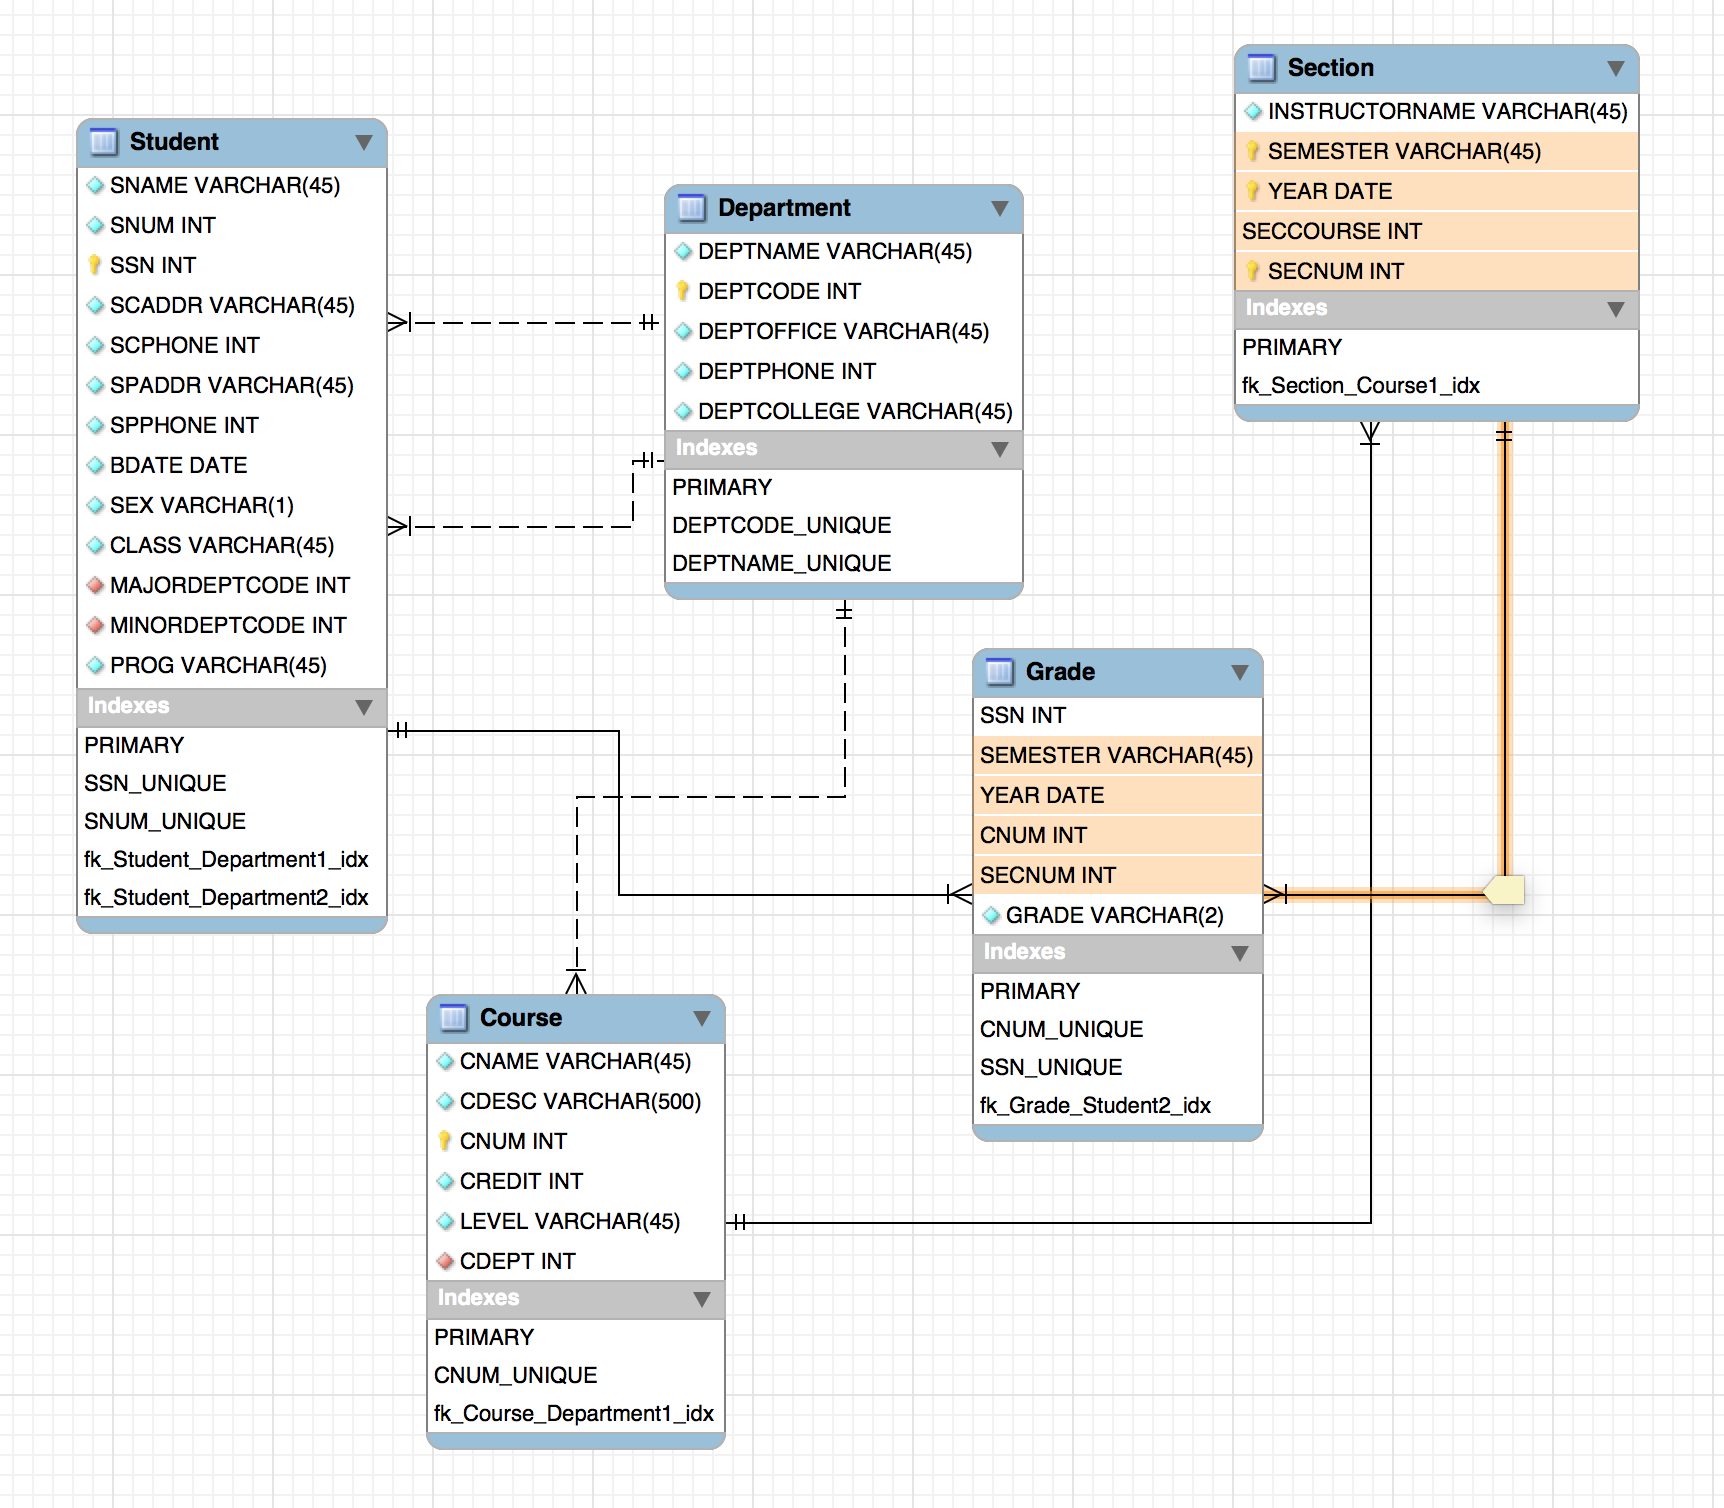
\includegraphics[scale=0.35]{erd.PNG}\\
			\end{center}

			\paragraph{}
				Starting with Student, there is a non-identifying one to many relationship between the foreign key Student.MAJORDEPTCODE and primary key Department.DEPTCODE as well as the foreign key Student.MINORDEPTCODE and primary key Department.DEPTCODE. This obviously allows us to relate the Student and Department entities and it is one to many because in Department DEPTCODE is determined to be unique and there could be many students with that major or minor department code. However, for every students department code major or minor there will only be one tuple within Department because again department codes are unique. There is also an identifying one to many relationship between Student.SSN and Grade.SSN. In the case of both it is the primary key and within DStudent a unique attribute, meaning the one tuple for every SSN can be related to the possibly many Grade tuples with that SSN. One will exist for every course that a student takes which is very likely to be greater than one. There is also a non-identifying one to many relationship between the primary key Department.DEPTCODE and the foreign key CDEPT. CDEPT is the attribute that holds the courses department number, that means that for every unique Department.DEPTCODE there will be many courses from that department in Courses that share department id's like all the classes in engineering etc. There is also an identifying one to many relationship between the primary key Courses.CNUM and the primary key Sections.SECCOURSE. In Courses every tuple has a unique course number CNUM and that will relate to the many sections of the same course. These will all share the same course number or Sections.SECCOURSE as they are the same course. Finally there is an identifying many to many relationship between Sections.{Semester, YEAR, SECCOURSE, SECNUM} and Grade.{SEMESTER, YEAR, CNUM, SECNUM}. These are all the same four values in each of the tuples in each entity. They are not unique in either entity which is why it is many to many. All of these attributes need to be related together as if both are not the same within the same tuple they will likely not be correctly related. For instance there are many sections with SECNUM 1 that have not relation between each other until they share the same course and section and are taught in the same year and semester.

		\subsection{MySQL Relational Model from ER Diagram}
			\paragraph{Student\\}
				\footnotesize{
					\begin{tabular}{| c | c | c | c | c | c | c |}
						\hline
						SNAME & SNUM & \underline{SSN} & SCADDR & SCPHONE & SPADDR & SPPHONE\\
						\hline
						BDATE & SEX & CLASS & \textcolor{red}{MAJORDEPTCODE} & \textcolor{red}{MINORDEPTCODE} & PROG & ---\\
						\hline
					\end{tabular}
				}

			\paragraph{Department\\}
				\footnotesize{
					\begin{tabular}{| c | c | c | c | c |}
						\hline
						DEPTNAME & \underline{DEPTCODE} & DEPTOFFICE & DEPTPHONE & DEPTCOLLEGE\\
						\hline
					\end{tabular}
				}

			\paragraph{Course\\}
				\footnotesize{
					\begin{tabular}{| c | c | c | c | c | c |}
						\hline
						CNAME & CDESC & \underline{CNUM} & CREDIT & LEVEL & \textcolor{red}{CDEPT}\\
						\hline
					\end{tabular}
				}

			\paragraph{Section\\}
				\footnotesize{
					\begin{tabular}{| c | c | c | c | c |}
						\hline
						INSTRUCTORNAME & \underline{SEMESTER} & \underline{YEAR} & \underline{SECCOURSE} & \underline{SECNUM}\\
						\hline
					\end{tabular}
				}

			\paragraph{Grade\\}
				\footnotesize{
					\begin{tabular}{| c | c | c | c | c | c |}
						\hline
						\underline{SSN} & \underline{SEMESTER} & \underline{YEAR} & \underline{CNUM} & \underline{SECNUM} & GRADE\\
						\hline
					\end{tabular}
				}

			\paragraph{}
				When generating the relational model we keep all the attributes and qualities of the ER diagram and simply change how the schema is represented. We underline primary keys and highlight in red foreign keys. I can not draw any arrows between tables in \LaTeX but the same connections from the ER diagram are applied here as well.

	\section{BCNF Database Schema \& Decomposition}
		Noting from section one Course, Section, and Grades are all already in BCNF since no other dependencies exist so that means those tables will not be changed from the way they are in the above relational model. That being said Student and department are not in BCNF and need to be decomposed.

		\begin{center}
			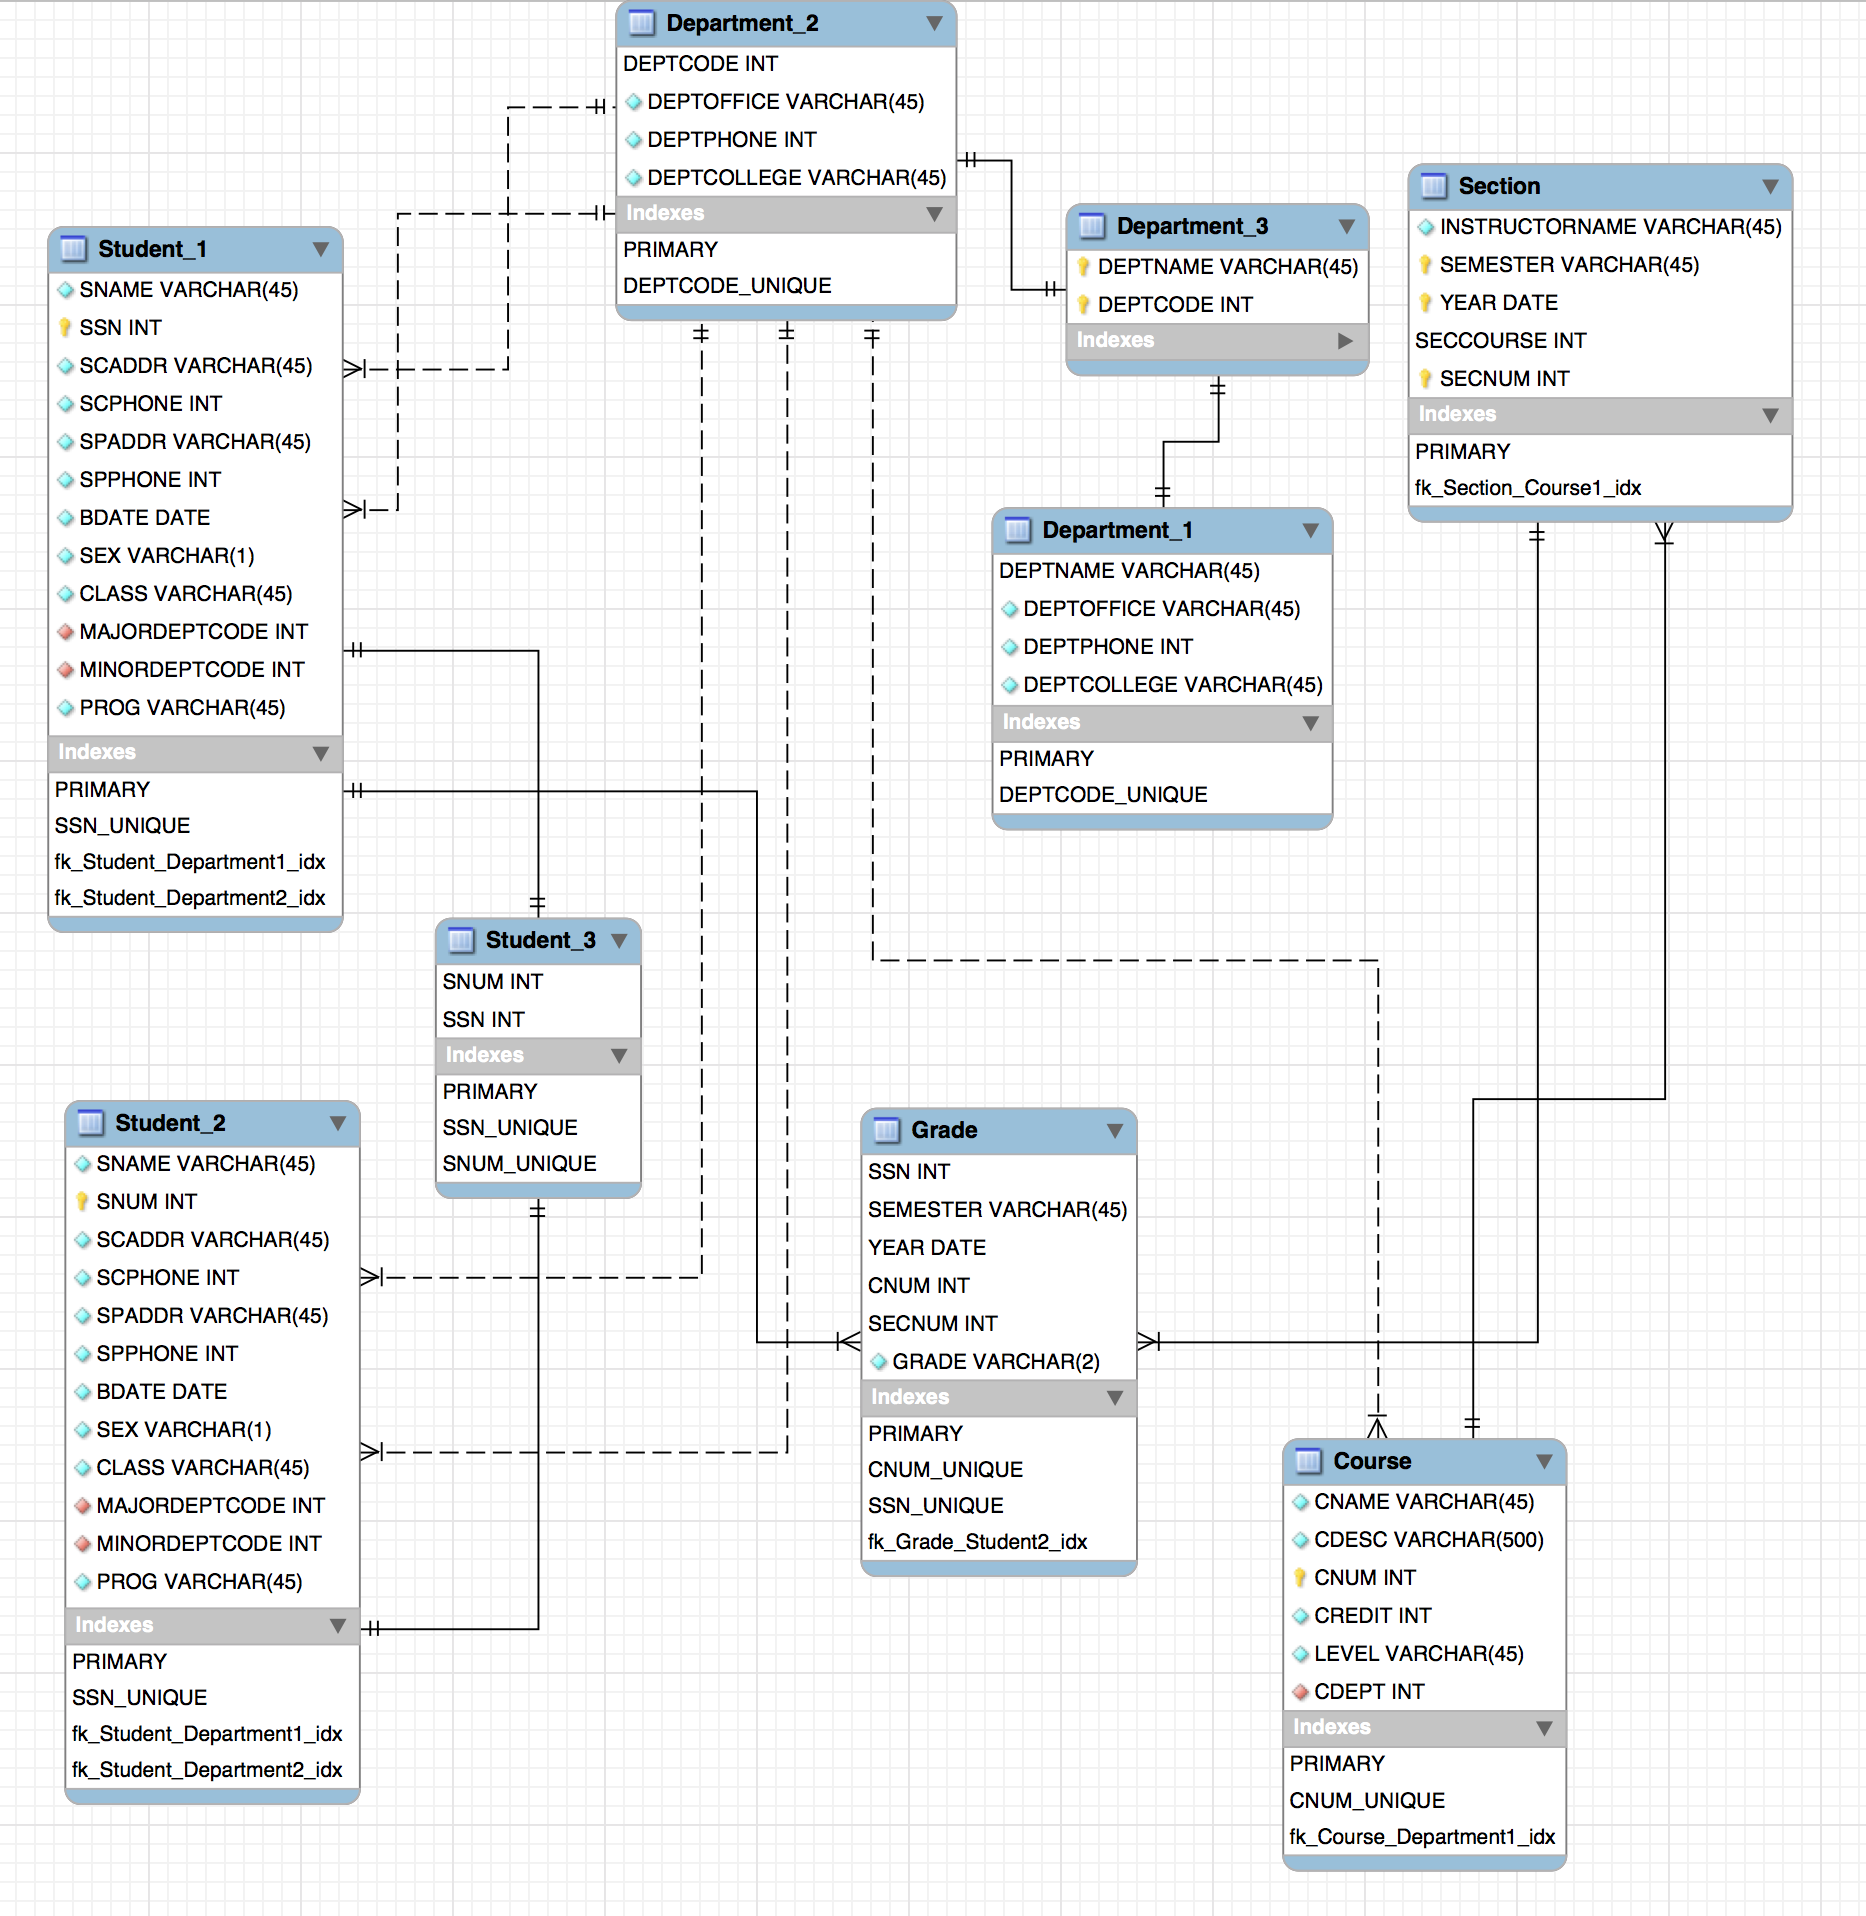
\includegraphics[scale=0.3]{bcnf.PNG}\\
		\end{center}

		\subsection{BCNF Decomposition}
			We will start with Student. In the case of student the only candidate key or minimal superkey is SNUM, SSN. There for both FDs are violating BCNF as they can not both be superkeys for Student. To perform the decomposition we make up a relation X and make it equal to Student. We then pick a FD that violates BCNF and add the relations to X. Finally we remove the dependency of the FD that we choose above from Student. The procdure is than repeated until there are no FDs that violate BCNF remaining, which in our case will be SNUM and SSN. What we are left with is two tables in the place of one, which is shown below. The other table that violates the BCNF is Department. In its case the only candidate key or superkey is DEPTNAME, DEPTCODE. To perform the decomposition on Department we do the same procedure that we used on Student. The returns two tables as well shown below.

		\subsection{BCNF Database Schema}
			\paragraph{Student\_1\\}
				\footnotesize{
					\begin{tabular}{| c | c | c | c | c | c |}
						\hline
						SNAME & \underline{SNUM} & SCADDR & SCPHONE & SPADDR & SPPHONE\\
						\hline
						BDATE & SEX & CLASS & \textcolor{red}{MAJORDEPTCODE} & \textcolor{red}{MINORDEPTCODE} & PROG\\
						\hline
					\end{tabular}
				}

			\paragraph{Student\_2\\}
				\footnotesize{
					\begin{tabular}{| c | c | c | c | c | c |}
						\hline
						SNAME & \underline{SSN} & SCADDR & SCPHONE & SPADDR & SPPHONE\\
						\hline
						BDATE & SEX & CLASS & \textcolor{red}{MAJORDEPTCODE} & \textcolor{red}{MINORDEPTCODE} & PROG\\
						\hline
					\end{tabular}
				}

			\paragraph{Student\_3\\}
				\footnotesize{
					\begin{tabular}{| c | c | c | c | c | c |}
						\hline
						\underline{SNUM} & \underline{SSN}\\
						\hline
					\end{tabular}
				}

			\paragraph{Department\_1\\}
				\footnotesize{
					\begin{tabular}{| c | c | c | c |}
						\hline
						\underline{DEPTNAME} & DEPTOFFICE & DEPTPHONE & DEPTCOLLEGE\\
						\hline
					\end{tabular}
				}

			\paragraph{Department\_2\\}
				\footnotesize{
					\begin{tabular}{| c | c | c | c |}
						\hline
						\underline{DEPTCODE} & DEPTOFFICE & DEPTPHONE & DEPTCOLLEGE\\
						\hline
					\end{tabular}
				}

			\paragraph{Department\_3\\}
				\footnotesize{
					\begin{tabular}{| c | c | c | c |}
						\hline
						\underline{DEPTNAME} & \underline{DEPTCODE}\\
						\hline
					\end{tabular}
				}

			\paragraph{Course\\}
				\footnotesize{
					\begin{tabular}{| c | c | c | c | c | c |}
						\hline
						CNAME & CDESC & \underline{CNUM} & CREDIT & LEVEL & \textcolor{red}{CDEPT}\\
						\hline
					\end{tabular}
				}

			\paragraph{Section\\}
				\footnotesize{
					\begin{tabular}{| c | c | c | c | c |}
						\hline
						INSTRUCTORNAME & \underline{SEMESTER} & \underline{YEAR} & \underline{SECCOURSE} & \underline{SECNUM}\\
						\hline
					\end{tabular}
				}

			\paragraph{Grade\\}
				\footnotesize{
					\begin{tabular}{| c | c | c | c | c | c |}
						\hline
						\underline{SSN} & \underline{SEMESTER} & \underline{YEAR} & \underline{CNUM} & \underline{SECNUM} & GRADE\\
						\hline
					\end{tabular}
				}

	\section{3NF Database Schema \& Sythesis}
		\begin{center}
			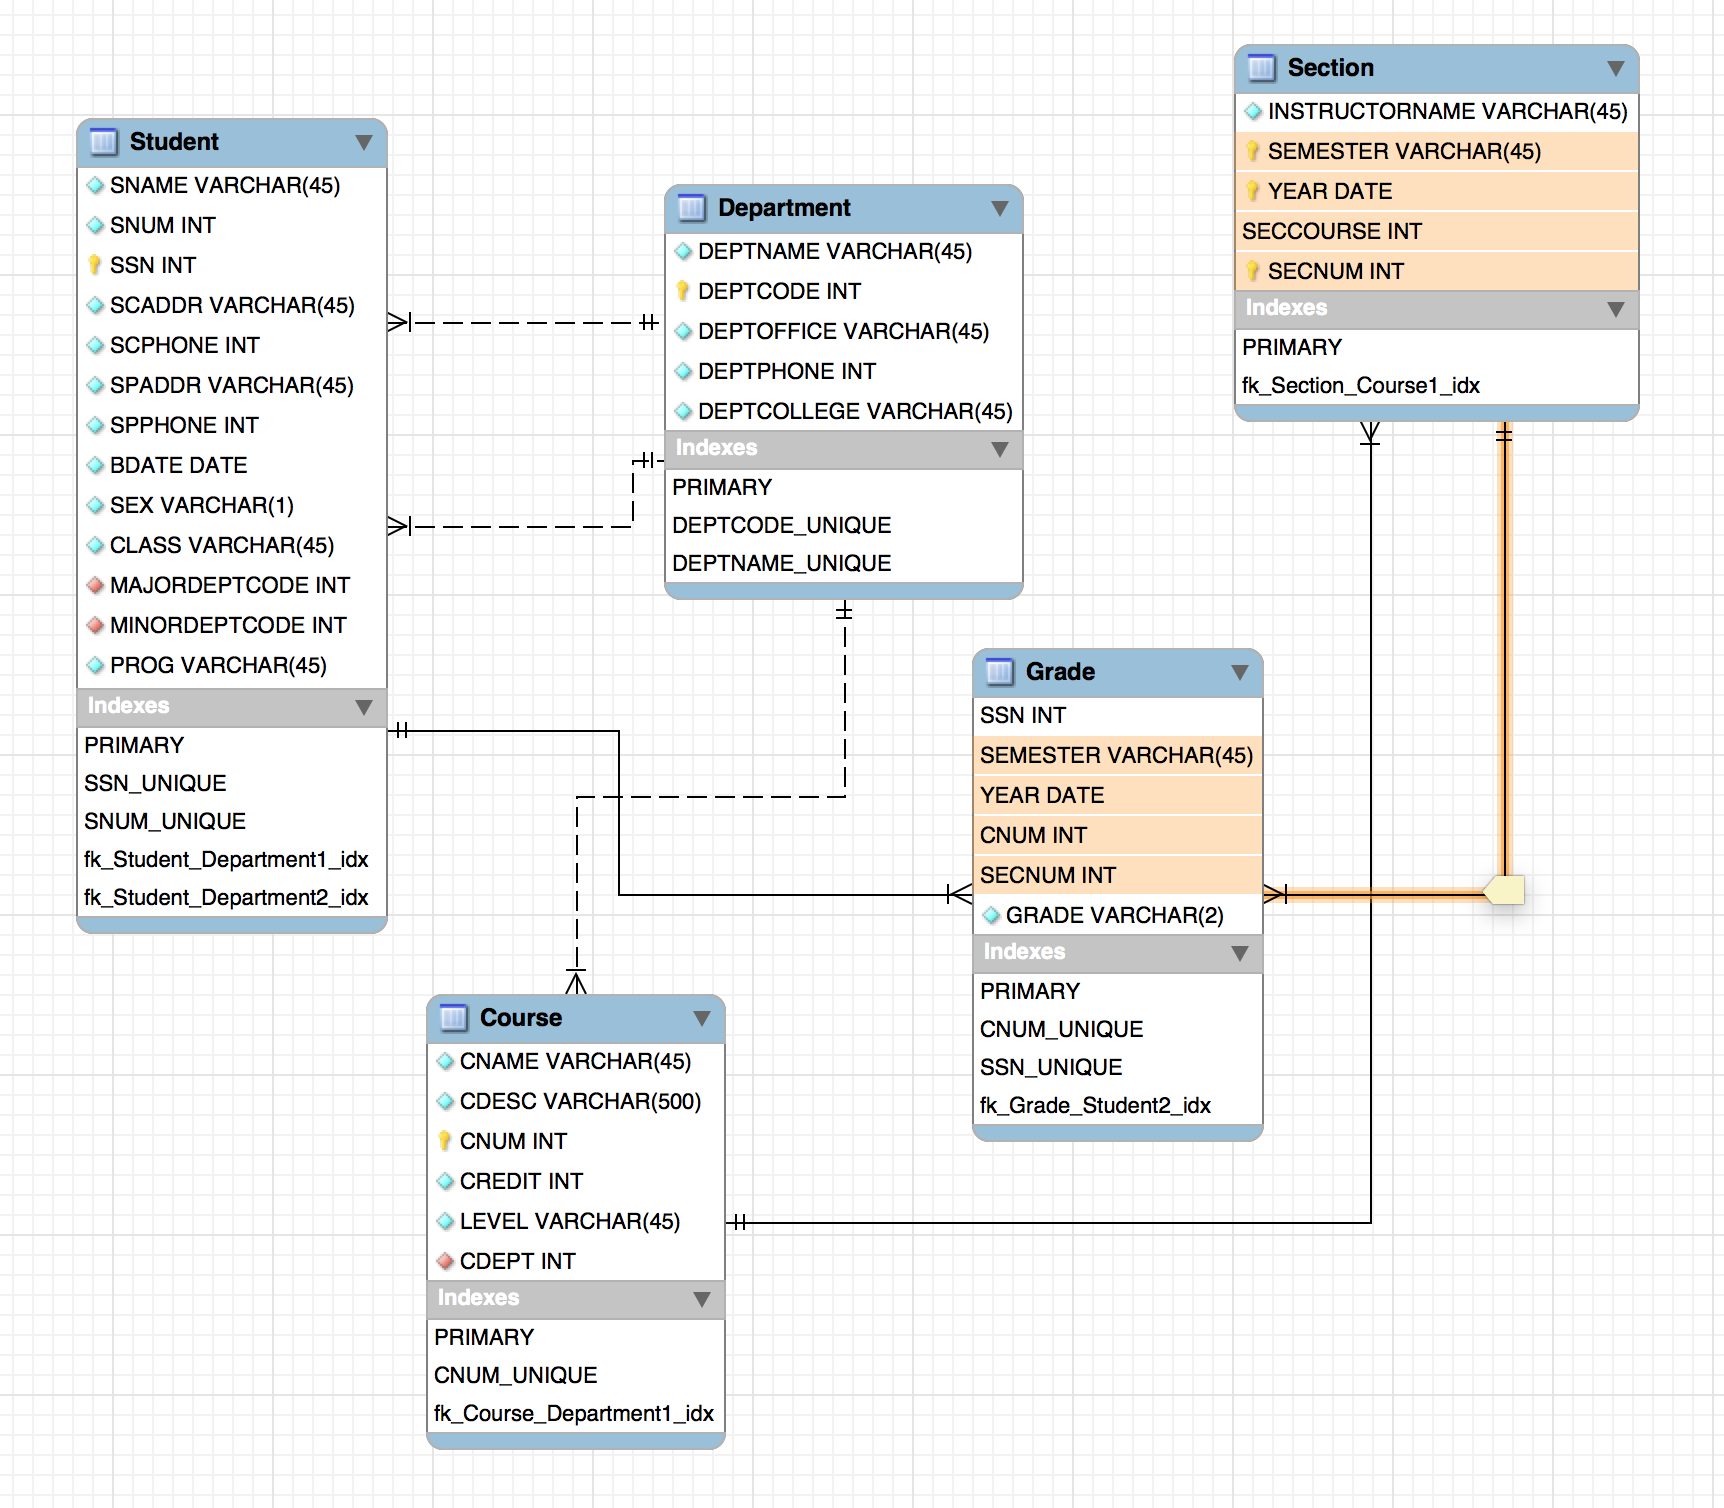
\includegraphics[scale=0.35]{erd.PNG}\\
		\end{center}

		\subsection{3NF Sythesis}
			To complete 3NF Synthesis we need to reduce any redundant FDs which we actually dont have to do since for Student and Department the only two tables with multiple FDs. Again just like in the BCNF decomposition the Course, Section, and Grade tables already will not violate 3NF, but Student and Department in fact do violate 3NF because of secondary keys. Once we have the FDs reduced and simplified if possible we can start to follow the synthesis algorithm, which would lead to one relation for every FD. The relation changes for Student and Department are shown below, which are just all the attributes in a non-redudant FDs. Once we have done that we check for any relations that are subsets of another since that would not also need to be included. Finally we ask if this final form allows for redundency? Due to the algorithm we used to get to this form, all of the attributes on the left side, SNUM, SSN, DEPTNAME, DEPTCODE, CNUM, SEMESTER, YEAR, SECCOURSE, and SECNUM, are they superkeys. You can see with the inclusion of SNUM and SSN in Student and DEPTNAME and DEPTCODE in Department that this form will violate BCNF so in fact allows for redundancy. Once we finish it ends up being the same as the original relational model because the duplicate FDs lead to duplicate relations so we can eliminate one of them and we are left with the same.

		\subsection{3NF Database Schema}
			\paragraph{Student\\}
				\footnotesize{
					\begin{tabular}{| c | c | c | c | c | c | c |}
						\hline
						SNAME & SNUM & \underline{SSN} & SCADDR & SCPHONE & SPADDR & SPPHONE\\
						\hline
						BDATE & SEX & CLASS & \textcolor{red}{MAJORDEPTCODE} & \textcolor{red}{MINORDEPTCODE} & PROG & ---\\
						\hline
					\end{tabular}
				}

			\paragraph{Department\\}
				\footnotesize{
					\begin{tabular}{| c | c | c | c | c |}
						\hline
						DEPTNAME & \underline{DEPTCODE} & DEPTOFFICE & DEPTPHONE & DEPTCOLLEGE\\
						\hline
					\end{tabular}
				}

			\paragraph{Course\\}
				\footnotesize{
					\begin{tabular}{| c | c | c | c | c | c |}
						\hline
						CNAME & CDESC & \underline{CNUM} & CREDIT & LEVEL & \textcolor{red}{CDEPT}\\
						\hline
					\end{tabular}
				}

			\paragraph{Section\\}
				\footnotesize{
					\begin{tabular}{| c | c | c | c | c |}
						\hline
						INSTRUCTORNAME & \underline{SEMESTER} & \underline{YEAR} & \underline{SECCOURSE} & \underline{SECNUM}\\
						\hline
					\end{tabular}
				}

			\paragraph{Grade\\}
				\footnotesize{
					\begin{tabular}{| c | c | c | c | c | c |}
						\hline
						\underline{SSN} & \underline{SEMESTER} & \underline{YEAR} & \underline{CNUM} & \underline{SECNUM} & GRADE\\
						\hline
					\end{tabular}
				}

	\section{Comparison Table of All Three Schemas}
		\subsection{Comparison Table}
			\begin{center}
				\begin{tabular}{| c | c | c | c |}
					\hline
					\textbf{---} & \textbf{ER Diagram} & \textbf{BCNF Decomposition} & \textbf{3NF Sythesis}\\
					\hline
					\textbf{Number of Tables} & 5 & 9 & 5\\
					\hline
					\textbf{Lossless} & Yes & Yes & Yes\\
					\hline
					\textbf{FDs Preserved} & Yes & No & Yes\\
					\hline
				\end{tabular}
			\end{center}

		\subsection{Explination}
			The ER Diagram/Relational Model is the baseline on the table with five tables and obviously loseless and preserving all FDs. Then when we performed the BCNF decomposition it is loseless, but does not preserve all of the FDs. For Student each table respectively losses the SNUM or SSN FD and for Department each table respectively losses the DEPTNAME or DEPTCODE FD. Also four tables are added, two for the decompression itself and two to relate the tables. When we follow the 3NF Synthesis algorithm described above we end up with duplicate added tables that we then remove and are left with the same schema, of course meaning that the relational model is in 3NF and therefore is loseless and preserves the FDs.
\end{document}